\chapter{Diseño de pruebas}
\section{Situaciones de prueba}
|WIP|

\section{Casos de prueba}
\begin{table}[H]
	\centering
	\begin{tabular}{l|c c c c c|c c|r r}
		\hline
		\multirow{2}*{\bf{ID}} & \multicolumn{5}{c|}{\textbf{Entradas}} & \multicolumn{2}{c|}{\bf{Totales}} & \multicolumn{2}{c}{\bf{Salidas}} \\
		\cline{2-10}
		& $BI_p$ & $BI_s$ & $R_p$ & $R_o$ & $P_{H}$ & $BI$ & $R$ & ¿Oblig.? & S. esperada \\
		\hline
		\hline
		CP1  & 0€      & 0€ & 0€ & 0€     & 0€ & 0€ & 0€ & No & TBA \\
		CP2  & 8999€   & 0€ & 0€ & 0€     & 0€ & 0€ & 0€ & No & TBA \\
		CP3  & 8999€   & 0€ & 0€ & 0€     & 0€ & 0€ & 0€ & Sí & TBA \\
		CP4  & 9000€   & 0€ & 0€ & 0€     & 0€ & 0€ & 0€ & Sí & TBA \\
		CP5  & 12449€  & 0€ & 0€ & $I-1$€ & 0€ & 0€ & 0€ & Sí & TBA \\
		CP6  & 12450€  & 0€ & 0€ & $I+1$€ & 0€ & 0€ & 0€ & Sí & TBA \\
		CP7  & 20199€  & 0€ & 0€ & $I$€   & 0€ & 0€ & 0€ & Sí & TBA \\
		CP8  & 20200€  & 0€ & 0€ & 0€     & 0€ & 0€ & 0€ & Sí & TBA \\
		CP9  & 35199€  & 0€ & 0€ & 0€     & 0€ & 0€ & 0€ & Sí & TBA \\
		CP10 & 35200€  & 0€ & 0€ & 0€     & 0€ & 0€ & 0€ & Sí & TBA \\
		CP11 & 59999€  & 0€ & 0€ & 0€     & 0€ & 0€ & 0€ & Sí & TBA \\
		CP12 & 60000€  & 0€ & 0€ & 0€     & 0€ & 0€ & 0€ & Sí & TBA \\
		CP13 & 299999€ & 0€ & 0€ & 0€     & 0€ & 0€ & 0€ & Sí & TBA \\
		CP14 & 300000€ & 0€ & 0€ & 0€     & 0€ & 0€ & 0€ & Sí & TBA \\
		\hline
	\end{tabular}
	\captionof{figure}{Casos de prueba iniciales propuestos para el sistema}
\end{table}

Los anteriores casos de prueba no cubren situaciones de validación de datos, ya que no se
considera relevante para este entregable teórico, para ello se definen algunos breves
ejemplos de validación de datos:
\begin{table}[H]
	\centering
	\begin{tabular}{l|c c c c c|c c|r r}
		\hline
		\multirow{2}*{\bf{ID}} & \multicolumn{5}{c|}{\textbf{Entradas}} & \multicolumn{2}{c|}{\bf{Totales}} & \multicolumn{2}{c}{\bf{Salidas}} \\
		\cline{2-10}
		& $BI_p$ & $BI_s$ & $R_p$ & $R_o$ & $P_{H}$ & $BI$ & $R$ & ¿Oblig.? & S. esperada \\
		\hline
		\hline
		CP91 & -1€   & 0€  & 0€    & 0€  & 0€  & -1€   & 0€    & \multicolumn{2}{c}{Error\cellcolor{red!25}} \\
		CP92 & 0€    & -1€ & 0€    & 0€  & 0€  & -1€   & 0€    & \multicolumn{2}{c}{Error\cellcolor{red!25}} \\
		CP93 & 0€    & 0€  & -1€   & 0€  & 0€  & 0€    & -1€   & \multicolumn{2}{c}{Error\cellcolor{red!25}} \\
		CP94 & 0€    & 0€  & 0€    & -1€ & 0€  & 0€    & -1€   & \multicolumn{2}{c}{Error\cellcolor{red!25}} \\
		CP95 & 9000€ & 0€  & 8900€ & 0€  & -1€ & 9000€ & 8900€ & \multicolumn{2}{c}{Error\cellcolor{red!25}} \\
		\hline
	\end{tabular}
	\captionof{figure}{Ejemplos de casos de prueba de validación de datos}
\end{table}

\section{Trazabilidad}
En esta sección se muestra la trazabilidad de los casos de prueba propuestos en la tabla anterior
con respecto a las situaciones de prueba definidas en la sección anterior.

Para facilitar su visualización y cumplir con los requisitos de la asignatura, ambas partes de
la tabla utilizan los identificadores únicos que facilitan su trazabilidad.

\begin{minipage}{\linewidth}
	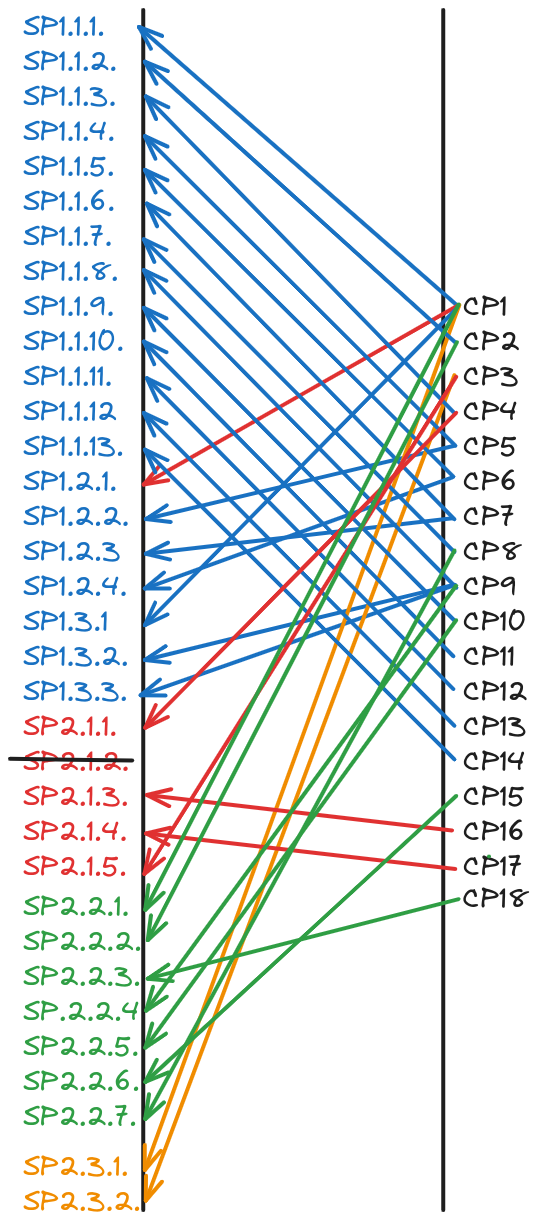
\includegraphics[width=\textwidth]{trazabilidad.png}
	\captionof{figure}{Trazabilidad del sistema}
\end{minipage}
